\section{Mischer}
\renewcommand{\ort}{topics/Mischer}

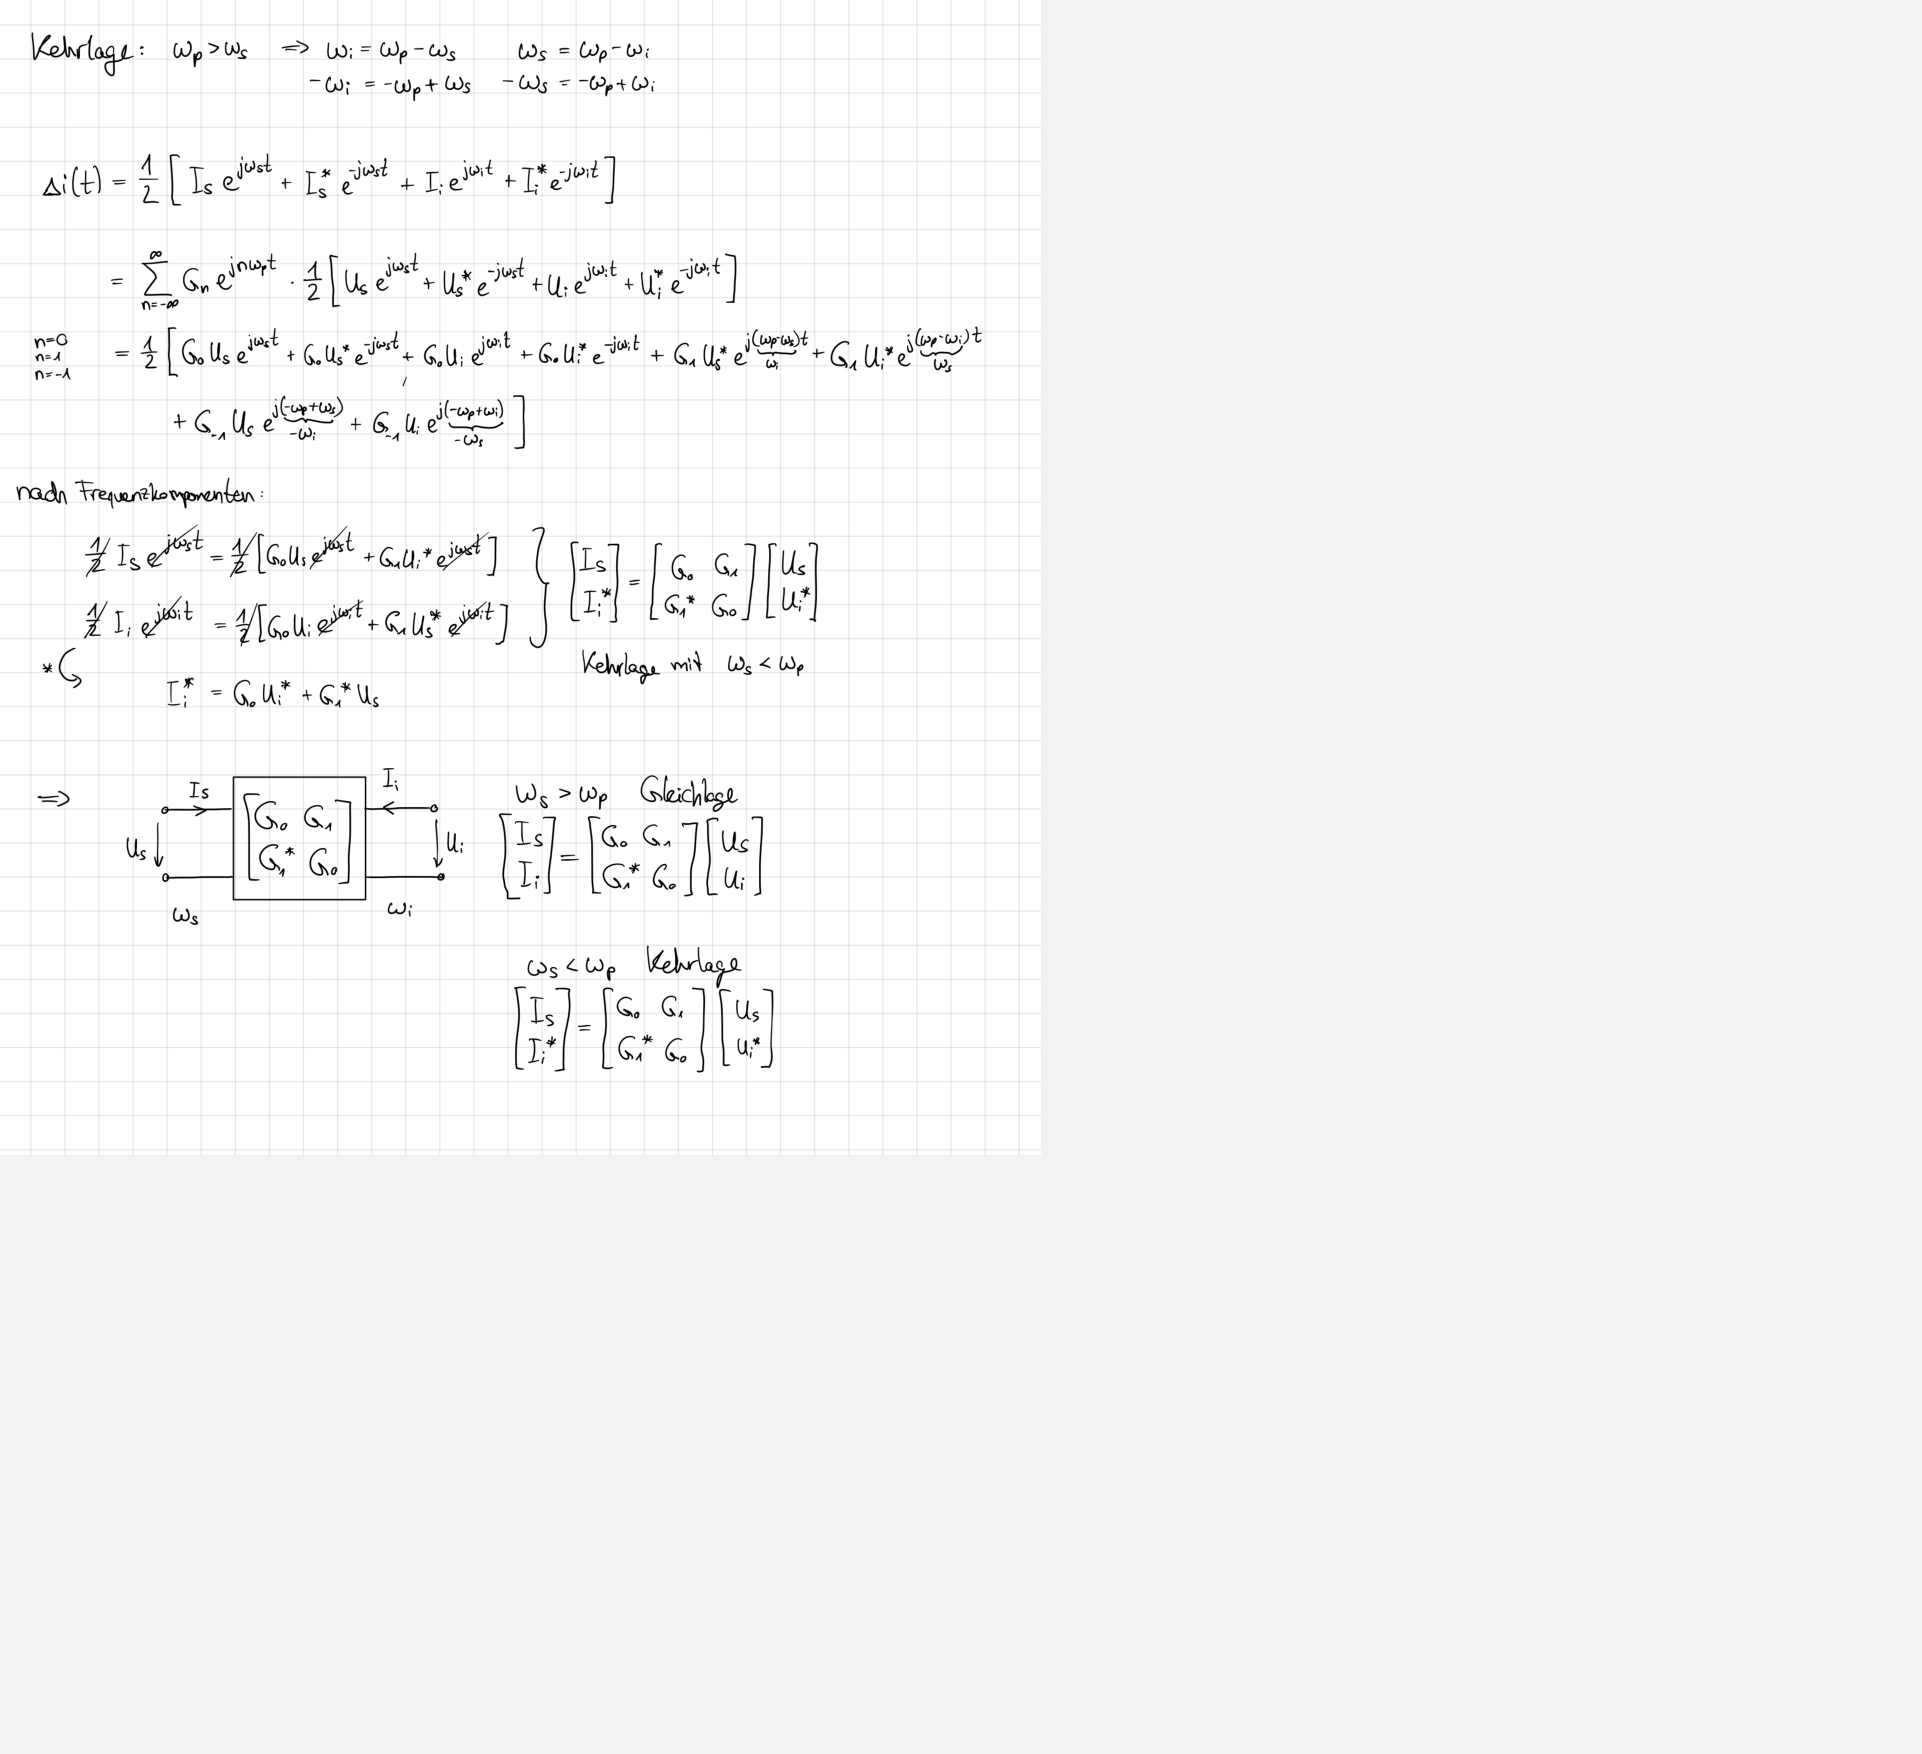
\includegraphics[width=\linewidth,page=1]{topics/Mischer/6. Mischer.pdf}
\includegraphics[width=\linewidth,page=2]{topics/Mischer/6. Mischer.pdf}

\subsection{Breitband-Mischer}

\bildf{BreitbandMischer}

\bildf{ESB BB Mischer}
$\begin{bmatrix}
    I_s \\ I_i \\ I^*_{sp}
\end{bmatrix} = \begin{bmatrix}
    G_0 & G_1 & G_2 \\ G_1^* & G_0 & G_1 \\ G_2^* & G_1^* & G_0 \\
\end{bmatrix} \begin{bmatrix}
    U_2 \\ U_i \\ U_sp^*
\end{bmatrix}$


\bildf{ESB Mischer}

$\begin{bmatrix}
    I_s \\ I_i
\end{bmatrix} = \begin{bmatrix}
    G_0 & G_1 \\ G_1^* & G_0
\end{bmatrix}\begin{bmatrix}
    U_s \\ U_i
\end{bmatrix}$


$I_sg = I_s + Y_s U_s$


$I_i = -Y_i U_i$

$\begin{bmatrix}
    I_{sg} \\ 0
\end{bmatrix} = \begin{bmatrix}
    G_0 + Y_s & G_1 \\ G_1^* & G_0 + Y_i
\end{bmatrix}\begin{bmatrix}
    U_s \\ U_i
\end{bmatrix}$

Gewinn $G_P = \frac{\text{Ausgangsleistung}}{\text{verfügbare Generatorleistung}}$

\bildf{verf Pgen}

$P_{g,av} = \frac{1}{2} \Re \{U_s I_s^*\}$

$U_s = \frac{I_{sg}}{Y_s + Y_s^*}$

$I_s = I_{sg} \frac{Y_s^*}{Y_s + Y_s^*}$

$\Rightarrow P_{g,av} = \frac{1}{2} \Re \left\{ \frac{I_{sg}I_{sg}^*Y_s}{(Y_s + Y_s^*)(Y_s + Y_s^*)^*}\right\}
= \frac{\abs{I_{sg}}^2}{8\Re \{Y_s\}}$

Ausgangsleistung: $P_2 = \frac{1}{2} \Re \{U_iI_i^*\} = \frac{1}{2} \Re \{U_iU_i^*Y_i\} = \frac{1}{2} \abs{U_i}^2 \Re\{Y_i\}$


$G_P = \frac{\frac{1}{2}\abs{U_i}^2 \Re\{Y_i\}}{\frac{1}{8}\abs{I_{sg}}^2 \frac{1}{\Re \{Y_s\}}}
= 4\abs{\frac{U_i}{I_sg}}^2 \Re\{Y_i\}\Re\{Y_s\}$


$\begin{bmatrix}
    U_s \\ U_i \end{bmatrix}= \begin{bmatrix}
        \tilde{G}
    \end{bmatrix}^{-1} \begin{bmatrix}
        I_{sg} \\ 0
    \end{bmatrix} = \frac{1}{(G_0 + Y_s)(G_0 + Y_i) - \abs{G_1}^2} \begin{bmatrix}
        G_0 + Y_i & -G_1 \\ -G_1^* & G_0 + Y_s
    \end{bmatrix} \begin{bmatrix}
        I_{sg} \\ 0
    \end{bmatrix}
$
$\frac{U_i}{I_{sg}} = \frac{-G_1^*}{(G_0 + Y_s)(G_0 + Y_i) - \abs{G_1}^2}$


$\Rightarrow G_P = 4 \frac{\abs{G_1}^2\Re\{Y_i\}\Re\{Y_s\}}{\abs{(G_0 + Y_s)(G_0 + Y_i) - \abs{G_1}^2}^2}$


\subsection{Ausführungsformen von Mischern}

\subsubsection{Ein Dioden Mischer}
\bildf{1DiodenMischer}

Elemente zu Verfügung
\begin{pitemize}
    \item \bildfR{0.1}{zimg1}
    \item \bildfR{0.1}{zimg2}
    \item \bildfR{0.1}{zimg4}
    \item \bildfR{0.1}{zimg3}
\end{pitemize}

\bildf{DiodeKS}


\subsubsection{Zwei Dioden Mischer}


\bildf{2DiodenMischer}


$u_p(t) = \hat{u}_p \cos(\omega_p t)$

$u_s(t) = \hat{u}_s \cos(\omega_s t + \varphi_s)$

Diode 1: $u_{D1}(t) \frac{1}{\sqrt{2}} \hat{u}_p \cos(\omega_p t) + \frac{1}{\sqrt{2}} \hat{u}_s \cos(\omega_s t + \varphi_s + 90^\circ)$

Diode 2: $u_{D2}(t) \frac{1}{\sqrt{2}} \hat{u}_p \cos(\omega_p t + 90^\circ) + \frac{1}{\sqrt{2}} \hat{u}_s \cos(\omega_s t + \varphi_s)$

$\Rightarrow u_i(t) = \kappa G_1 \hat{u}_s \cos\left((\omega_s - \omega_p)t + \varphi_s  90^\circ\right)$

$u_i(t) = \kappa G_1 \hat{u}_s \cos\left( \omega_i t + \varphi_s + 90^\circ\right)$


Einfach balancierter Mischer
Rauschbalancierung $\Rightarrow$ Amplitudenschwankungen eben sich auf durch guten Gleichlauf der Dioden.
und ihre entgegengesetzt orientierte Einbaurichtung.

\subsubsection{4-Dioden-Mischer}


\bildf{4DiodenMischer}

ZF$-$Phase resultiert als Differenzphase hier all ZF$-$Pfeile.
Parallel $Rightarrow$ summieren sich auf.
\begin{pitemize}
    \item Rauschbalancierung $\rightarrow$ Amplitudenschwankungen heben sich auf.
    \item Signalbalancierung: RF$-$LO, RF$-$ZF, LO$-$ZF, da alle Tore entkoppelt sind.
\end{pitemize}


Für höherfrequente Realisierung $\Rightarrow$ Einsatz von Kopplern

\bildf{4DiodenMischer mit RK}


Phasenregelkreise
\begin{pitemize}
    \item Synthesegenerator
    \item Stabilisierung von Signalen
\end{pitemize}



Skalar Netzwerkanalysator

\bildf{skalarNWA}

Vektorielle Netzwerkanalysatoren

\bildf{vektorNWA}


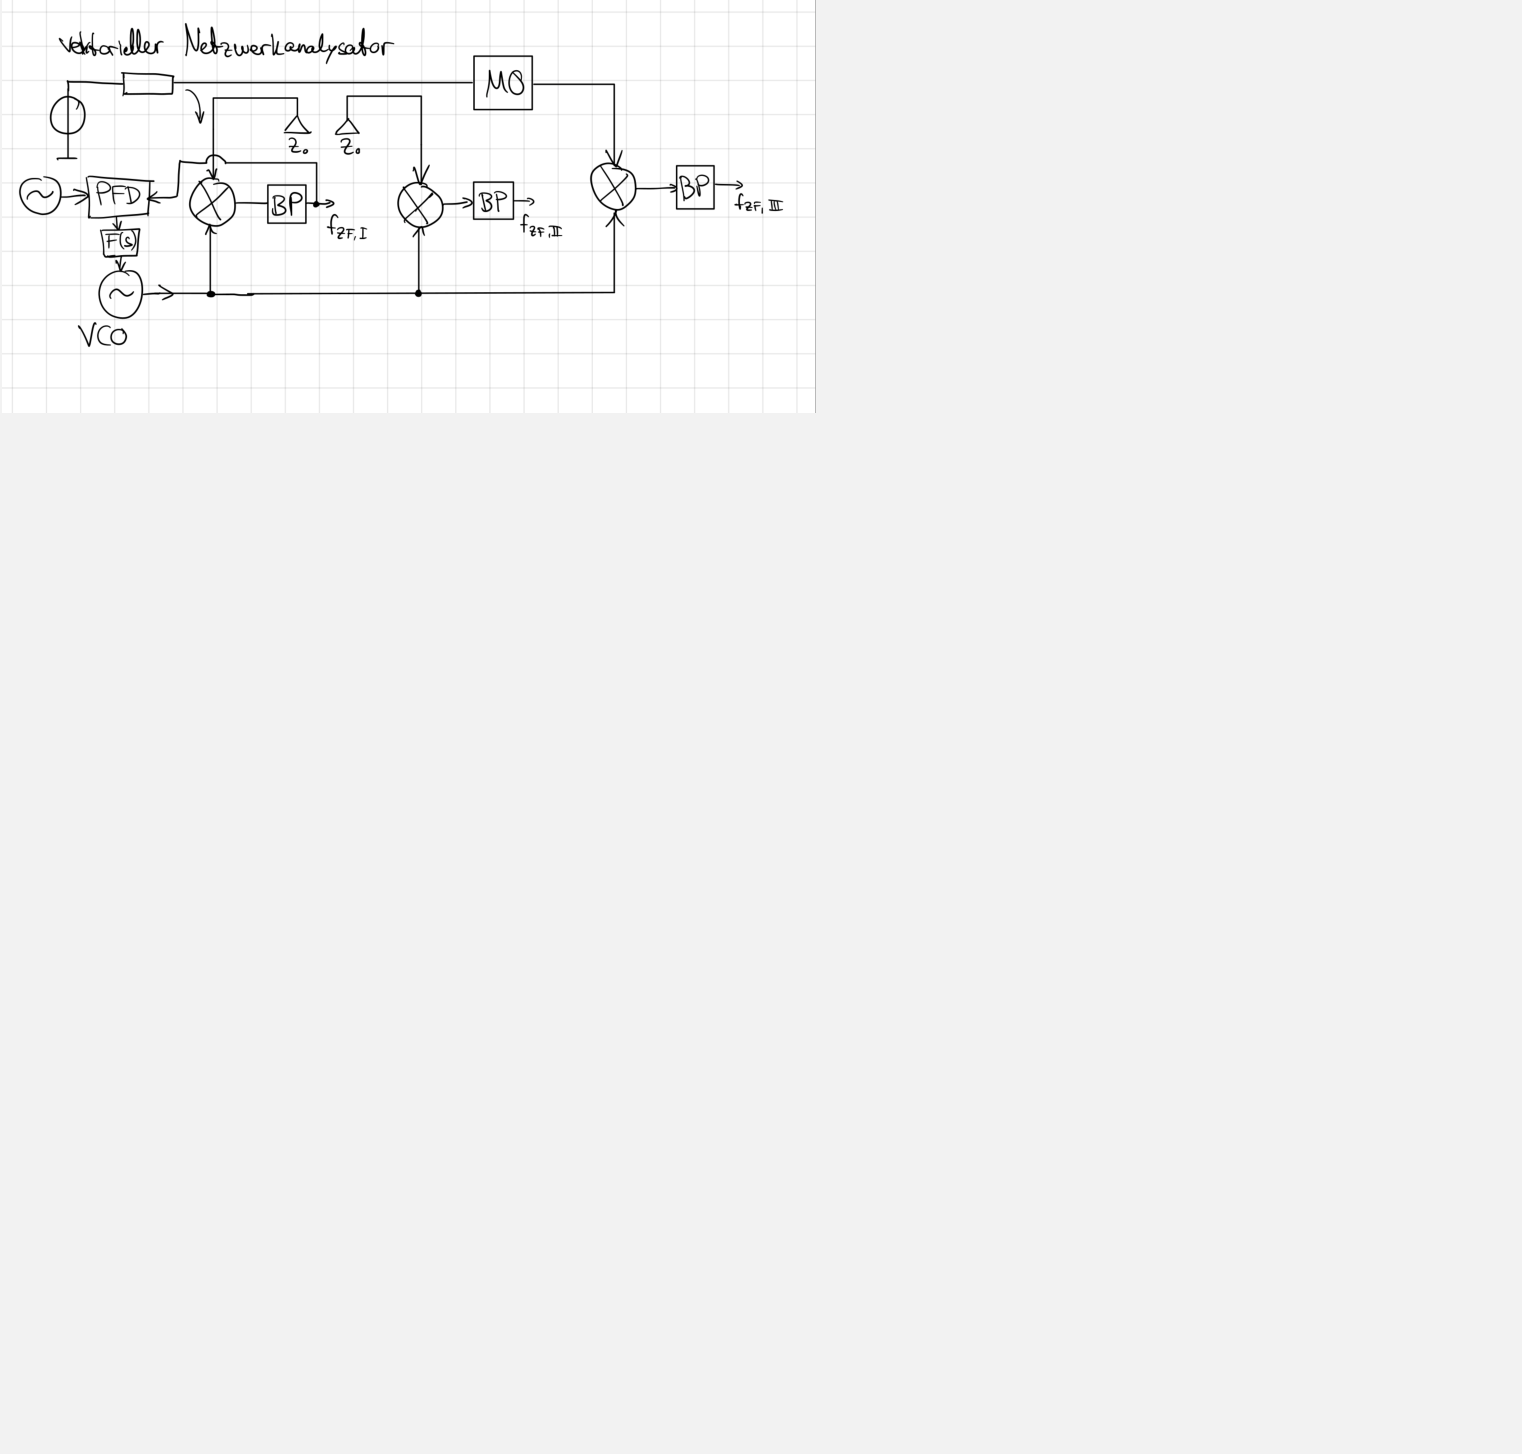
\includegraphics[width=\linewidth,page=1]{topics/Mischer/7.Phasenregelkreise.pdf}
\includegraphics[width=\linewidth,page=2]{topics/Mischer/7.Phasenregelkreise.pdf}
\includegraphics[width=\linewidth,page=3]{topics/Mischer/7.Phasenregelkreise.pdf}
\includegraphics[width=\linewidth,page=4]{topics/Mischer/7.Phasenregelkreise.pdf}




\subsection{Digitale Phasendiskriminatoren}

\subsubsection{Exklusiv Oder- Gatter}

$I_R^V$ Xor Y

\begin{tabular}{cc|c}
    R & V & Y\\
    0 & 0 & 0\\
    0 & 1 & 1\\
    1 & 0 & 1\\
    1 & 1 & 0
\end{tabular}

Vor.: Tastverhältnis der Signale 50\%

\fb \\

$\theta_e = \theta_R - \theta_V$

stabiler Regelpunkt bei $90^\circ$: 
\begin{itemize}
    \item Nicht seitenbandselektiv.
    \item Recktecksingale mit 50\% Tastverhältnis
\end{itemize}


\subsubsection{Flip Flop als unsymmetris. PD}

\fb \\

S = Set 
R = Reset 

\fb FF\\

\fb Die 9 Plots. \\ 

\fb Plot von Uq und Theta e\\

\begin{itemize}
    \item seitenbandselektiv
    \item flankengesteuert
\end{itemize}


\subsection{Phasen-Frequenz-Diskriminatoren PFD}

\fb Shaltbild\\

Zustandgraph:\\

\begin{pitemize}
    \item $\uparrow 0 \hat{=}$ Flanke am Ref. Eingang.
    \item $0 \uparrow \hat{=}$ Flanke am VCO Eingang.
    \item $00 \hat{=}$ Keine Flanke.
    \item $\uparrow \uparrow \hat{=}$ Flanke am Ref. und VCO Eingang.
\end{pitemize}

$U_q = A-B$

3 Zustände $\Rightarrow$ frequenzselektiv
$K_d = \frac{U_h}{2 \pi}$


\subsection{Schritt-/Synthesegeneratoren}
\fb \\

\begin{pitemize}
    \item Reproduzierbare Frequenzeinstellung
    \item Kleine Einschwingzeit für schnelle Einstellung
    \item Kleines $\Delta f$ für lineare Rampe
    \item Optimales Phasenrauschen
\end{pitemize}


\subsubsection{Einschleifiger Phasenregelkreis}
Realisierung eines Schrittgenerators

\fb \\

\begin{pitemize}
    \item $\Delta f = f_{Ref}$
    \subitem $\Delta f \downarrow \rightarrow f_{Ref} \downarrow \rightarrow N \uparrow$
    \item Phasenrauschen des VCO
    \subitem $W_V \sim N^2$
    \item Eckfrequenz des Regelkreises $F(s)$
    \subitem $f_c \approx \frac{1}{20} f_{Ref}$
    \subitem $f_{Ref} \downarrow \rightarrow f_c \downarrow \rightarrow$ Langsames Einschwingungsverhalten
\end{pitemize}


\subsubsection{PLL mit Mischer}

\fb \\

\begin{pitemize}
    \item $f_V = f_{Lo} \pm N f_{Ref}$
    \item $\Delta f_V = f_{Ref}$
    \item Kleinere Teilungsfaktor $\rightarrow$ geringeres Phasenrauschen
    \item keine Reduktion der Frequenzschrittweite
\end{pitemize}

\subsubsection{Verschachtelte PLL}

\fb \\


\begin{pitemize}
    \item $f_z = \abs{f_v - f_{v2}}$
    \item $f_{v2} = L f_{Ref}$
    \item $f_{v3} = N f_{Ref}$
    \item $f_{v3} = M f_{z} $
    \item $f_v = f_{v2} \pm f_z = L \cdot f_{Ref} \pm \frac{N \cdot f_{Ref}}{M}$
    \item $\Delta f_v = \frac{f_{Ref}}{M}$
\end{pitemize}


\subsection{PLL mit fraktionalem Teiler}

\fb Schaltbild\\

\fb N über Zeit\\

\begin{pitemize}
    \item M Takte einer Periode T
    \item Zeitl. Mittelwert: $\bar{N} = \frac{(M - k)N + k(N + 1)}{M} = N + \frac{k}{M}$
    \item $f_v = (N + \frac{k}{M}) f_{Ref}$
\end{pitemize}          

Frequenzrampe
\fb Frequenzrampe \\

wirkt wie zufälliges "Umschalten" des Teilungsfaktor $\rightarrow$ noise shaping $\rightarrow$ um Störsignale zu unterdrücken, die bei periodischen umschalten erscheinen.

\fb Spektrum \\

\fb Frequenzrampe \\

\begin{pitemize}
    \item N wird im gleichen Zeitabständen $\Delta T$ verändert
    \item Bandbreite $B = f_{max} - f_{min} = N_{max} f_{Ref} - N_{min} f_{Ref} = Zf_{Ref} $
    \item Rampendauer: $T = Z \Delta T = Z \frac{1}{f_{Ref}}$
    \item $BT = Z^2 \Leftrightarrow Z = \sqrt{BT}$
\end{pitemize}



